%%%%%%%%%%%%%%%%%%%%%%%%%%%%%%%%%%%%%%%%%%%%%%%%%%%%%%%%%%%%%%%%%%%%%%%%%%%%%%%%
%2345678901234567890123456789012345678901234567890123456789012345678901234567890
%        1         2         3         4         5         6         7         8

\documentclass[letterpaper, 10 pt, conference]{ieeeconf}  % Comment this line out if you need a4paper

%\documentclass[a4paper, 10pt, conference]{ieeeconf}      % Use this line for a4 paper

\IEEEoverridecommandlockouts                              % This command is only needed if 
                                                          % you want to use the \thanks command

\overrideIEEEmargins                                      % Needed to meet printer requirements.

% See the \addtolength command later in the file to balance the column lengths
% on the last page of the document

% The following packages can be found on http:\\www.ctan.org
%\usepackage{graphics} % for pdf, bitmapped graphics files
%\usepackage{epsfig} % for postscript graphics files
%\usepackage{mathptmx} % assumes new font selection scheme installed
%\usepackage{times} % assumes new font selection scheme installed
%\usepackage{amsmath} % assumes amsmath package installed
%\usepackage{amssymb}  % assumes amsmath package installed
\usepackage{graphicx}
\usepackage[export]{adjustbox}
\graphicspath{ {images/} }


\title{\LARGE \bf
DuckieMVP - a path-planning, cooperative, interactive, heterogeneous, K-12 multi-robots system
}


\author{Eric Lu$^{1}$ Wei-Chen Lei$^{2}$ Kuang-Yen Li$^{3}$% <-this % stops a space
\thanks{*This work was supported by the Robotics Master Program in National Chiao Tung University, Taiwan}% <-this % stops a space
\thanks{$^{1}$Eric Lu
        {\tt\small eric565648@gmail.com}}%
\thanks{$^{2}$Wei-Chen Lei,
        {\tt\small sean0514.eed04@nctu.edu.tw}}%
\thanks{$^{2}$Kuang-Yen Li,
        {\tt\small dalek669528@gmail.com}}%
}


\begin{document}



\maketitle
\thispagestyle{empty}
\pagestyle{empty}


\section{INTRODUCTION \& MOTIVATION}

Imaging a big factory, if we want the factory be smart enough, there must be some robots that can pick and place and even move something gigantic together.

About path-planning or manipulation or multi-robot system, there are many existing platform. For example, MicroMVP$^{1}$ is a platform that focusing on multi-robot behavior and Pheeno$^{2}$ is a robot that focus on manipulation while moving and can do cooperative manipulation. However, none of them can do path-planning and cooperative manipulation at the same time. Therefore, we want to build a system that the user can do the path planning and task planning, while the robot can follow the commands to move to the right place and do cooperative manipulation. By this, we can make a factory much more intelligent.

Also, we will add Scratch in this project. Since programming of K12 is popular and get more attention worldwide. We plan to let the user program though Scratch.

\section{SYSTEM ARCHITECTURE \& EQUIPMENTS}

\subsection{SYSTEM ARCHITECTURE}
The DuckieMVP including three parts, motion capture camera, center control computer and robots. (Fig. 1) The whole system acts like aliens controlled by a center-control, powerful "brain" in movies. The whole system is based on Robot Operating System ,Duckietown and MicroMVP.
\begin{figure}[h] % h means put this image here
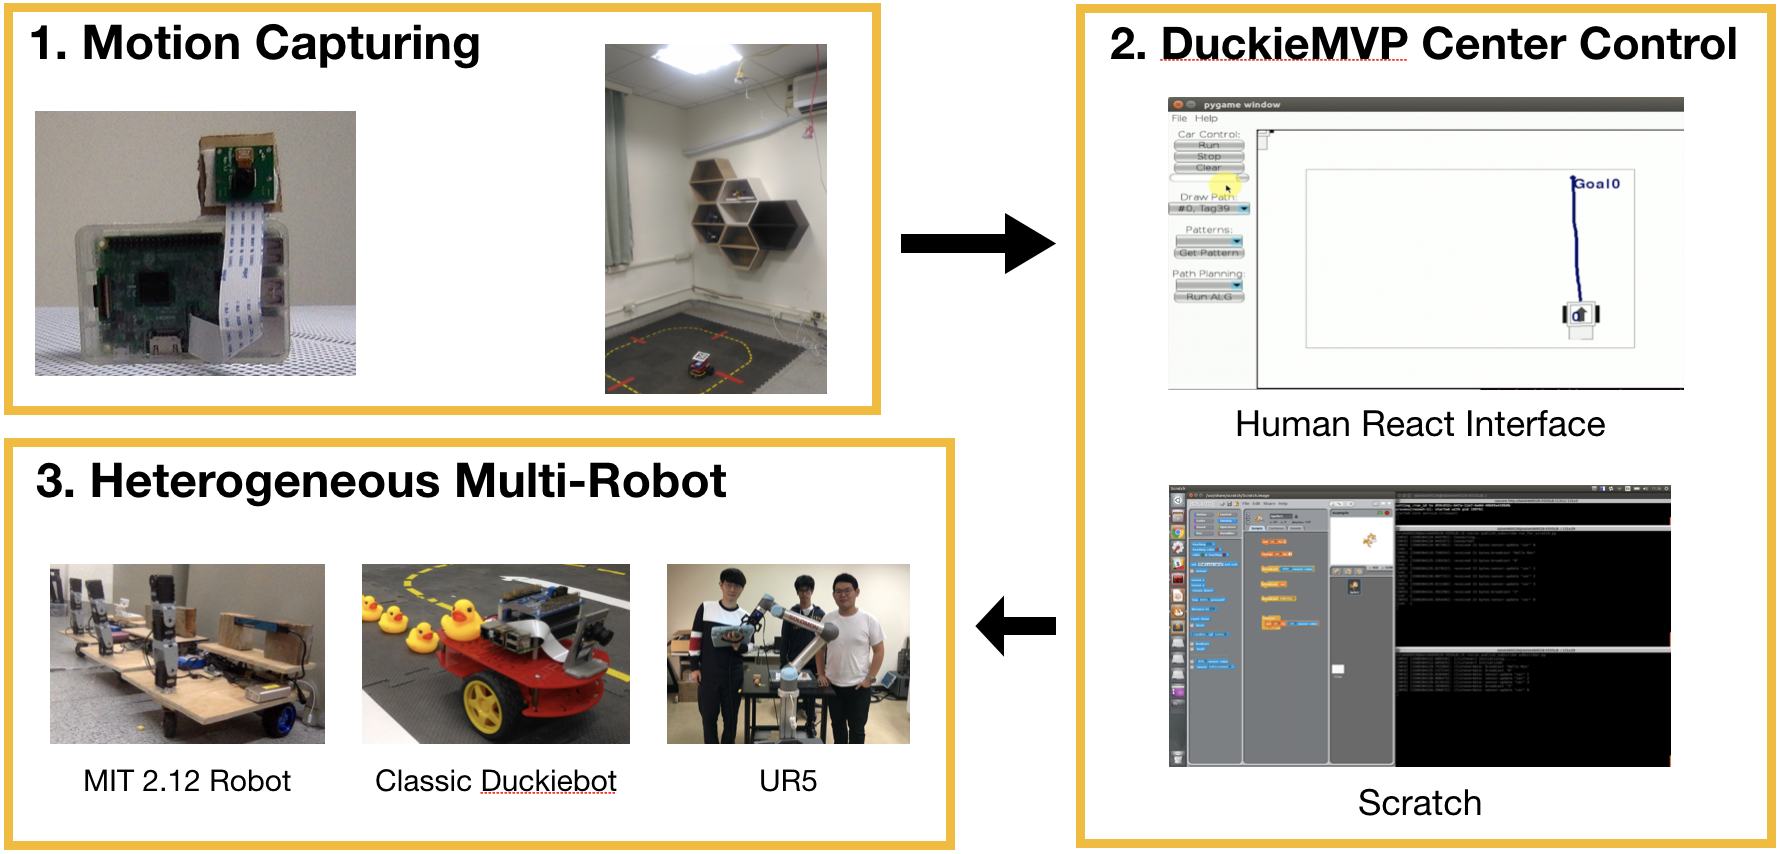
\includegraphics[width=1\columnwidth]{system_diagram1}
\centering
\caption{The basic system diagram of DickieMVP}
 \label{figure:system_diagram1}
\end{figure}

The function of the motion-capture camera is to capture images from above which contains two-dimensional bar codes that specifies the locations of robots.  The camera is connected with computer with ethernet.

The most important part in DuckieMVP is the center control computer. Before all the algorithm and commands, the control center will get images from camera and decode the tags to find out the locations of each robots. After calculating and decision making, the control center will send commands to robots. For end user, there's a panel for user to interact and add commands to the system. Three main functions will be add to the control system. First, it can produce a trajectory for robots to follow, which is one of the crucial parts in the system. After producing a trajectory, an algorithm will compute the thrusts of right and left wheels for robots to receive and follow the path while the robots are differential drive robots (DDR). Second, the control system can compute a trajectory for a fleet of robots to follow. A fleet do not just follow the trajectory randomly, but will follow the trajectory according to some center of the mass. Third, the robots can cooperatively manipulate an object.

Each of the robots is basically a differential drive robots (DDR) with a gripper. They act like slaves of the control center. It will get every command from the center including thrust of motors and movement of the grippers. The robots will be looked over by motion-capture camera and form a closed-loop control system.
\begin{figure}[h] % h means put this image here
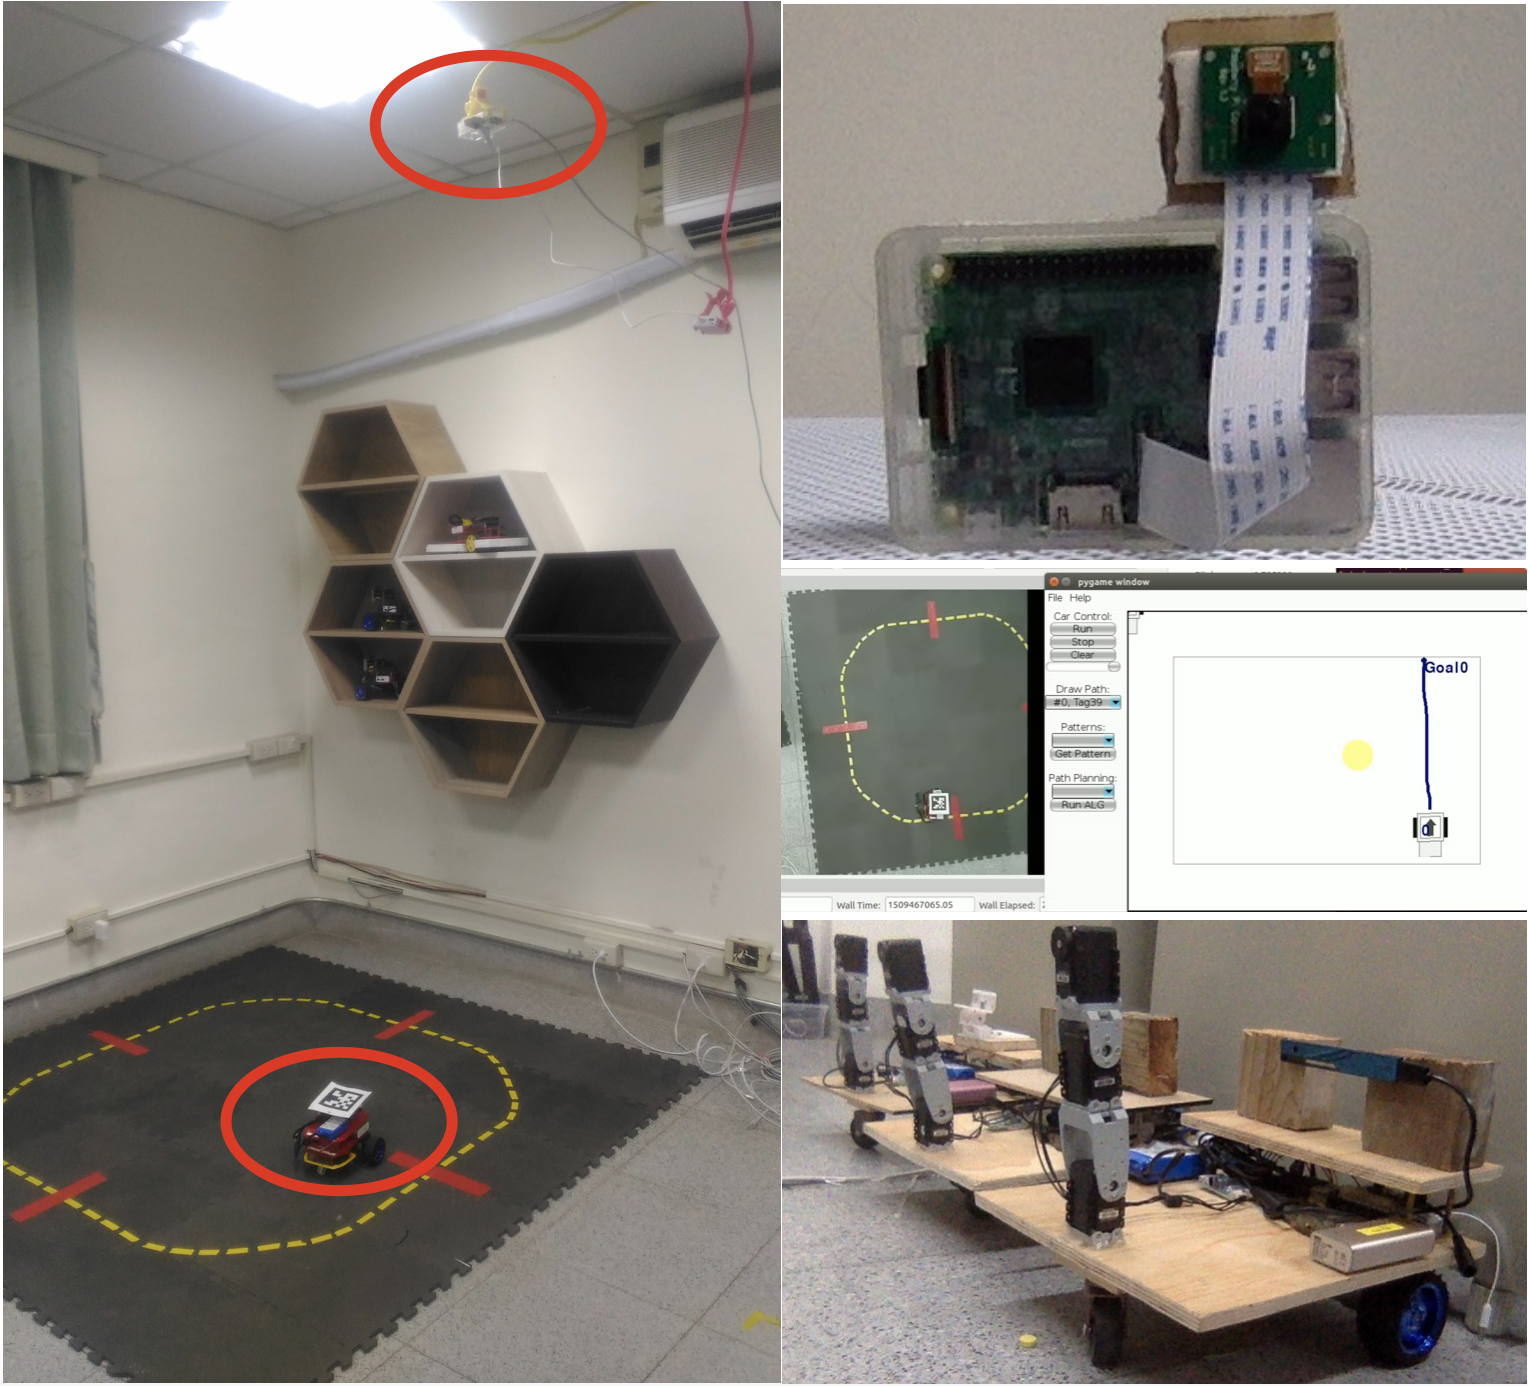
\includegraphics[width=1\columnwidth]{system_diagram_pic}
\centering
\caption{The photo of hardware setup and components}
 \label{figure:system_diagram_pic}
\end{figure}

\subsection{EQUIPMENTS} 

The camera is composed of a Raspberry Pi 3 and a camera without fisheye lens. (Fig. 3) The camera will connect with control center through ethernet. 
\begin{figure}[h] % h means put this image here
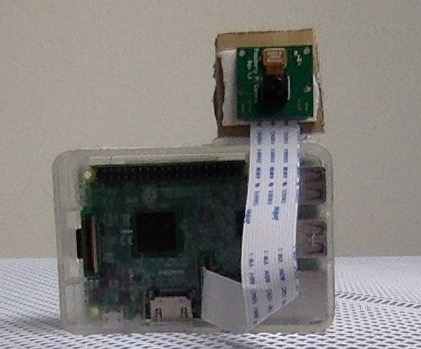
\includegraphics[width=0.8\columnwidth]{mocap}
\centering
\caption{Motion capture system: a camera with a Rpi3}
 \label{figure:mocap}
\end{figure}

The control center is an ordinary computer with an CPU of i5 and without GPU. (Fig. 4) There's a interactive panel for user. Also, we will set up scratch interface for programming.
\begin{figure}[h] % h means put this image here
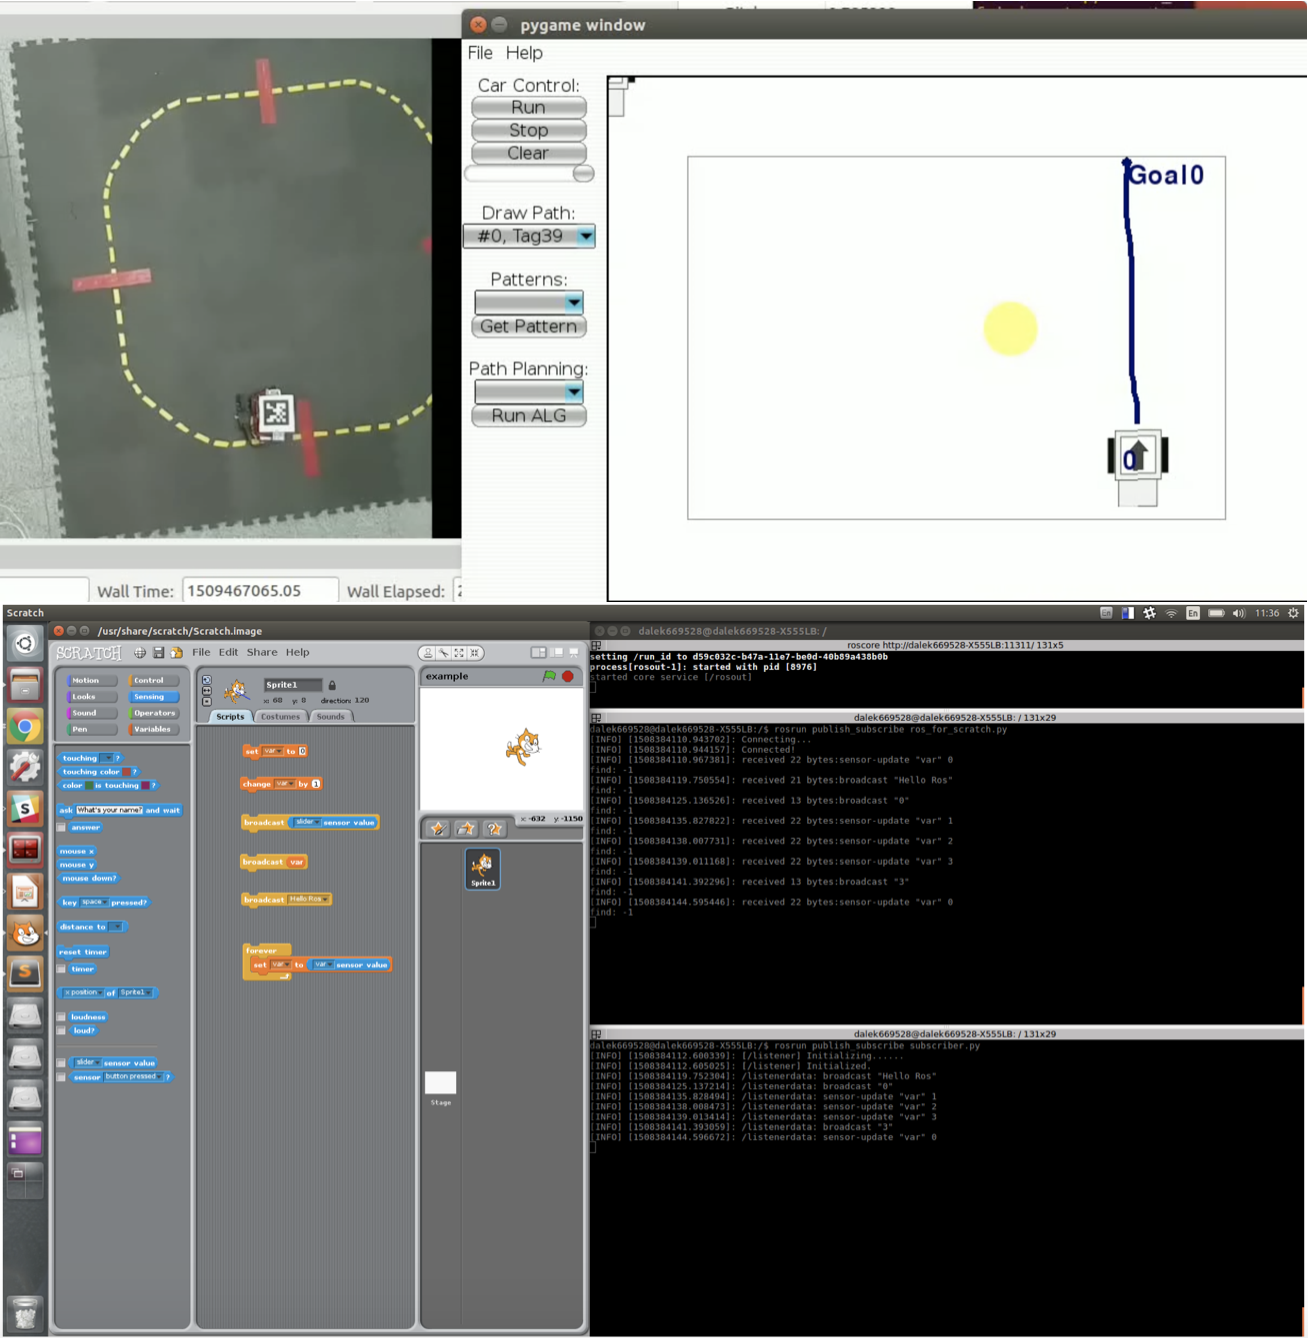
\includegraphics[width=0.8\columnwidth]{interface}
\centering
\caption{The interface of DuckieMVP and Scratch for programming.}
 \label{figure:interface}
\end{figure}

About the robots, we will take MIT 2.12 lab robots with a three axis arm and gripper as reference. (Fig. 5) We may modify the robots to suit our need. Of course, Duckiebot DB17 will definitely be part of the project. Classic never loss!
\begin{figure}[h] % h means put this image here
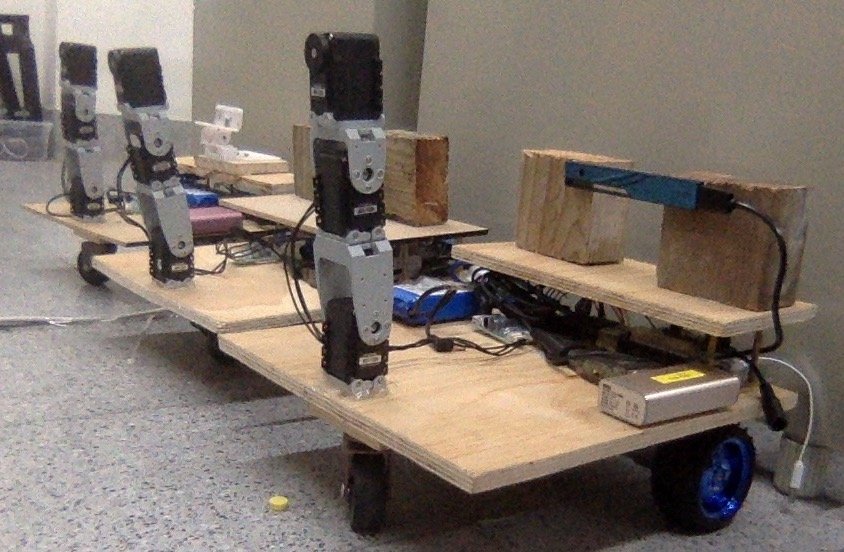
\includegraphics[width=0.8\columnwidth]{robot}
\centering
\caption{The MIT 2.12 robot. We will modify a little bit to suit our usage.}
 \label{figure:robot}
\end{figure}
\begin{figure}[h] % h means put this image here
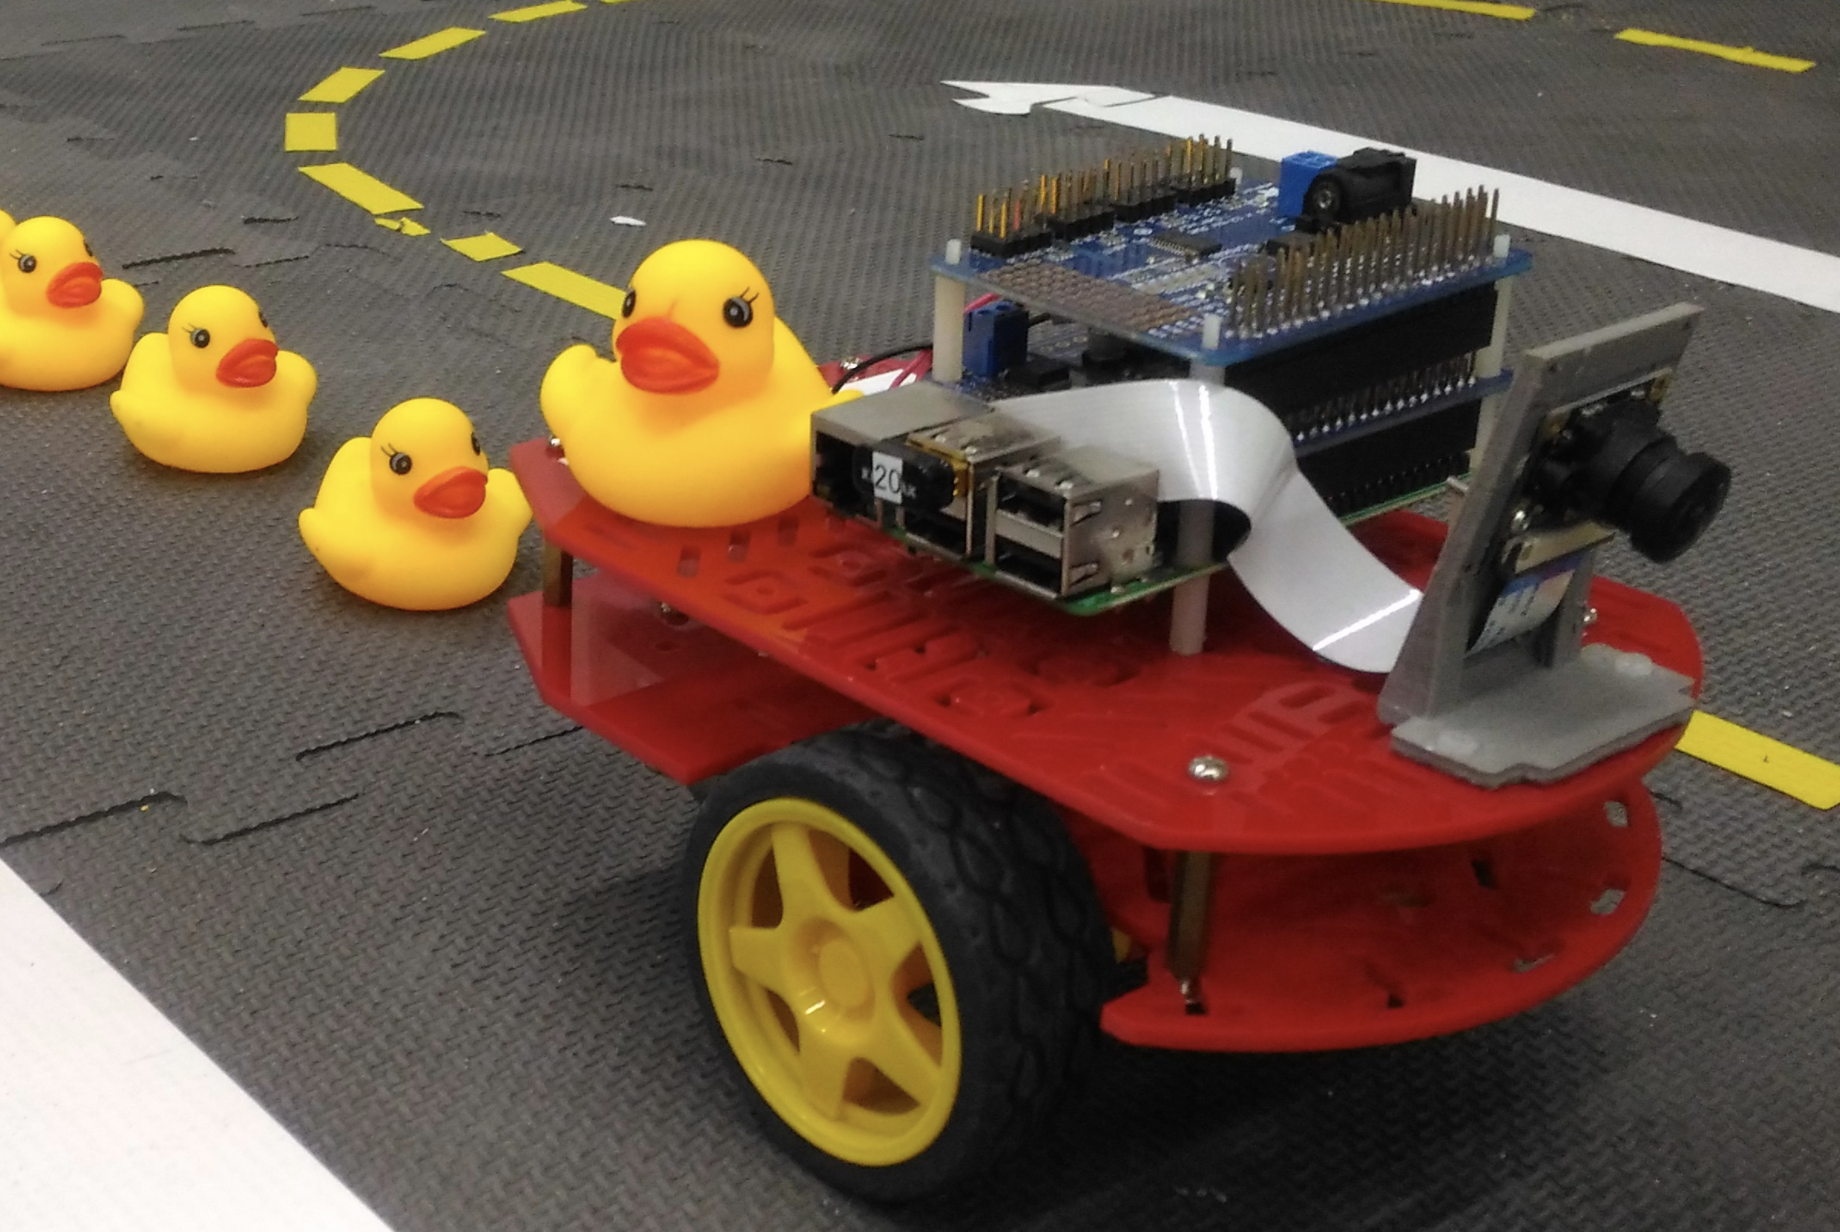
\includegraphics[width=0.95\columnwidth]{DB17}
\centering
\caption{Duckiebot DB17. Classic never loss!}
 \label{figure:DB17}
\end{figure}

\section{SPECIFIC AIMS}

\begin{itemize}
\item The robots can follow a trajectory by the commands from control center individually.
\item The center of mass of a fleet of robots can follow the trajectory
\item Robots can cooperatively manipulate an object.
\item Users can use the system through Scratch and create education value
\item Building an easy-to-use interface enable all level of end user.
\end{itemize}

\section{APPROACH}

DuckieMVP is based on Robot Operating System which will reduce the connection problem. For the apriltag detection, we will take the package in Duckietown as reference. We will create a new package in Duckietown workspace so that we can take advantage of original Duckietown packages. The commands interface and DDR algorithm will be transplanted from MicroMVP and added into DuckieMVP package. Also, the algorithm of fleet control will be implemented inside the DuckieMVP package. 

For Scratch, we know that there's a way for Scratch communicate with ROS node, and already make a prototype. We wil build an interface for user can control system through Scratch programming.

\section{SCHEDULE AND TEAM COLLABORATION}

We plan to complete the project in about two months. The whole project is divided into three parts, the basic trajectory following, trajectory followed by fleets and cooperative manipulation. We plan to finish the basic trajectory following in first week since we have started the project already. Then, we will use four weeks to study on how the fleet can following the trajectory and implement the function. After that we will spend last four weeks on cooperative manipulation. We will integrate the previous function to achieve our goal.

\begin{thebibliography}{1}

\bibitem{IEEEhowto:kopka}
Jingjin Yu, Shuai D. Han, Wei N. Tang, and Daniela Rus, \emph{"A Portable, 3D-Printing Enabled Multi-Vehicle
Platform for Robotics Research and Education"}, IEEE Robotics and Automation (ICRA) 2017.
\bibitem{IEEEhowto:kopka}
Sean Wilson, Ruben Gameros, Michael Sheely, Matthew Lin, Kathryn Dover, Robert Gevorkyan, Matt Haberland, Andrea Bertozzi, and Spring Berman, \emph{"Pheeno, A Versatile Swarm Robotic Research and Education Platform"}, IEEE Robotics and Automation (ICRA) 2016.
\bibitem{IEEEhowto:kopka}
Liam Paull, Jacopo Tani, Heejin Ahn, Javier Alonso-Mora, Luca Carlone, Michal Cap, Yu Fan Chen,
Changhyun Choi, Jeff Dusek, Yajun Fang, Daniel Hoehener, Shih-Yuan Liu, Michael Novitzky, Igor Franzoni
Okuyama, Jason Pazis, Guy Rosman, Valerio Varricchio, Hsueh-Cheng Wang, Dmitry Yershov, Hang Zhao,
Michael Benjamin, Christopher Carr, Maria Zuber, Sertac Karaman, Emilio Frazzoli, Domitilla Del Vecchio,
Daniela Rus, Jonathan How, John Leonard, and Andrea Censi, \emph{"Duckietown: an Open, Inexpensive and Flexible
Platform for Autonomy Education and Research"}, IEEE Robotics and Automation (ICRA) 2017.

\end{thebibliography}


\addtolength{\textheight}{-12cm}   % This command serves to balance the column lengths
                                  % on the last page of the document manually. It shortens
                                  % the textheight of the last page by a suitable amount.
                                  % This command does not take effect until the next page
                                  % so it should come on the page before the last. Make
                                  % sure that you do not shorten the textheight too much.

\bibliographystyle{IEEEtran}
\bibliography{egbib}

\end{document}
